\documentclass[11pt]{article}

\usepackage[utf8]{inputenc}
\usepackage[danish]{babel}
\usepackage[T1]{fontenc}
\usepackage{float}
\usepackage{fancyhdr}
\usepackage{amsmath}
\usepackage{color}
\usepackage[export]{adjustbox}
\usepackage{graphicx}
\usepackage{lastpage}
\usepackage{enumitem}
\usepackage{wrapfig}
\usepackage[a4paper, top = 1in, bottom = 1in, left=1in,right=1in]{geometry}
\usepackage[hidelinks]{hyperref}

\hfuzz=500pt

\newcommand{\tabitem}{~~\llap{\textbullet}~~}

\newcommand{\resumeSubheading}[4]{
  \noindent\begin{tabular*}{0.98\textwidth}[t]{l@{\extracolsep{\fill}}r}
    \noindent \textbf{#1} & #2 \\ \vspace{-3pt} 
    \noindent \textit{\small#3} & \textit{\small #4} 
  \end{tabular*}\vspace{7pt}
}

\newcommand{\listitem}[2]{
  {\small{\tabitem{#1}}} & {\small\tabitem{#2}}\\
}

\begin{document}
\begin{center}
  \textbf{\huge{\scshape{Peter Heilbo Ratgen}}}\\ 
  \vspace{0.2cm}
  \small 31330916 $|$
  \href{mailto:peter@pratgen.dk}{\underline{peter@pratgen.dk}} $|$
  \href{https://github.com/PeterRatgen }{\underline{github}} $|$
  \href{https://pratgen.dk}{\underline{pratgen.dk}} $|$
  \href{https://www.linkedin.com/in/peter-ratgen-a1236529/}{\underline{linkedin}}
\end{center}

\noindent\large{\scshape{Om mig}} \newline
\noindent{\rule[0.3cm]{\textwidth}{0.4pt}}

\begin{wrapfigure}{R}{0.22\textwidth}
  \vspace{-0.7cm}
  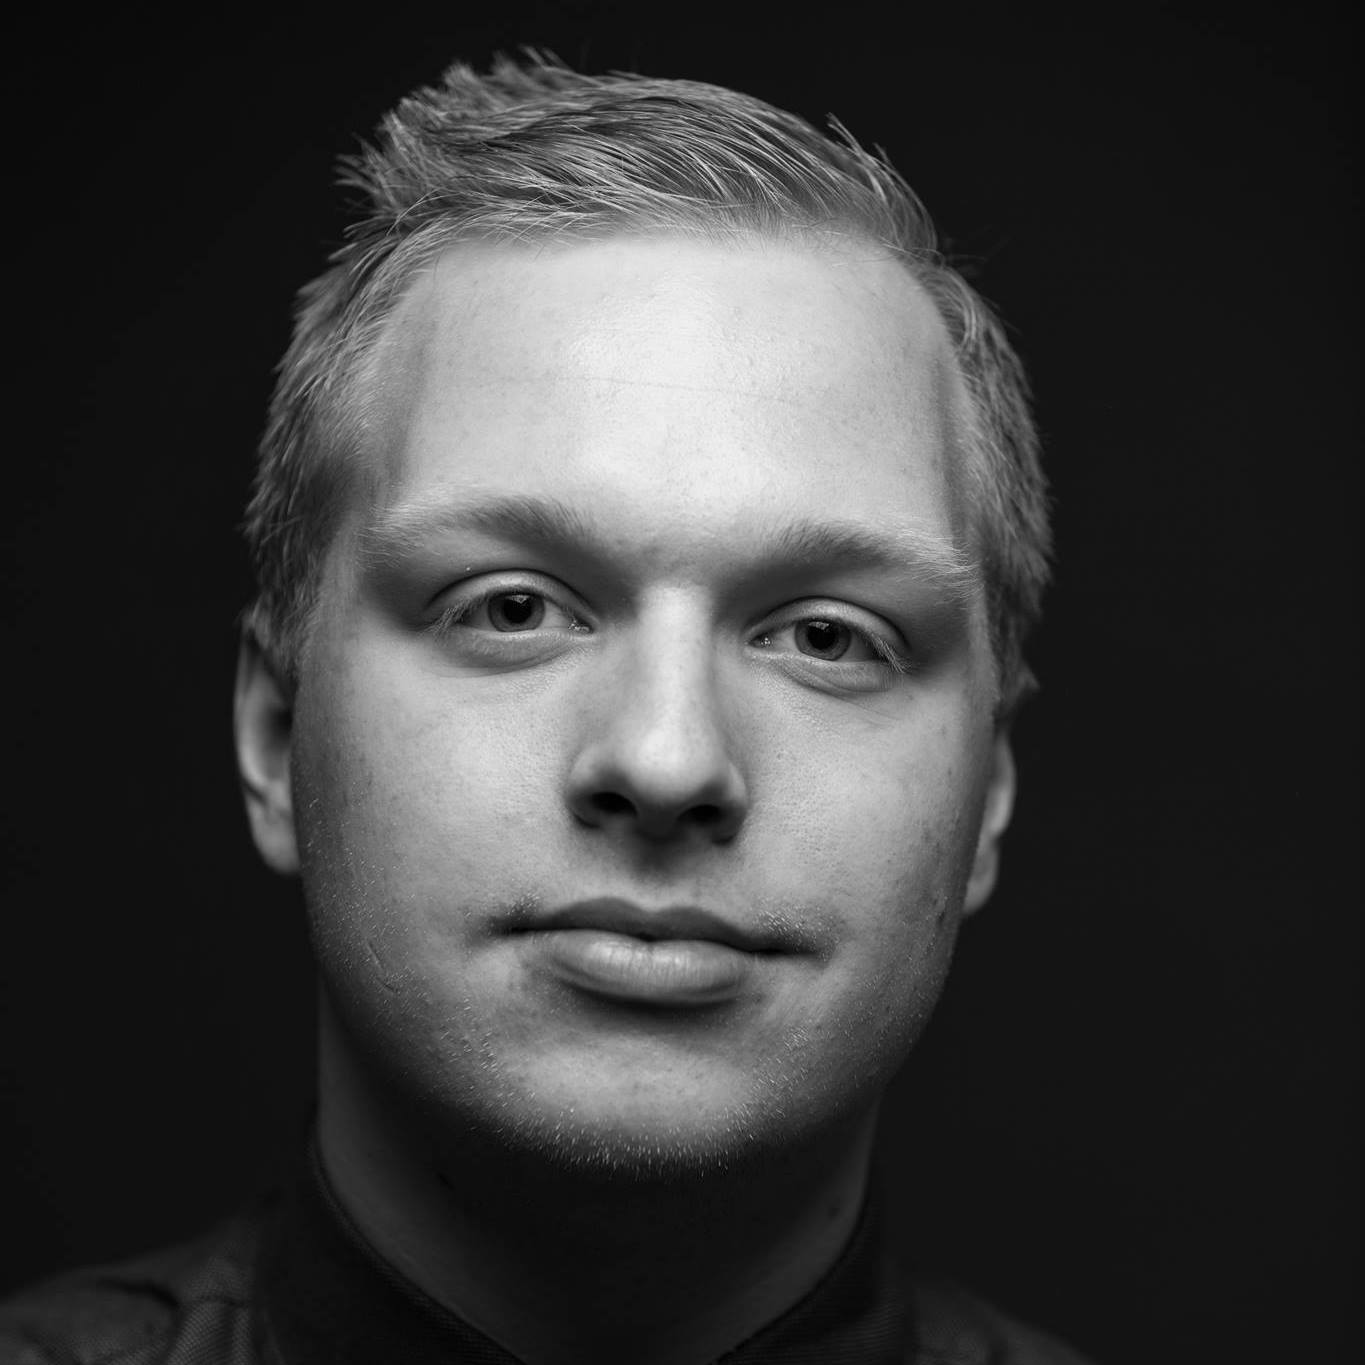
\includegraphics[width=0.2\textwidth, right]{./okay.jpg}
\end{wrapfigure}
\normalsize Software Engineering studerende, tidligere Datalogi studerende, bor
i Odense, jeg er 22 år gammel. Jeg er en drevet person, der elsker at dykke ned
i projekter, om det er projekter på universitet eller mine egne. Jeg har en stor
interesse i at lære nye færdigheder, samt at øge min produktivitet igennem nye
og spændende værktøjer. Jeg er særligt interesseret i at arbejde med back-end,
samt at arbejde med Linux.

\vspace{0.3cm}
\noindent\large{\scshape{Uddannelse}} \newline
\noindent{\rule[0.3cm]{\textwidth}{0.4pt}}

\resumeSubheading{Syddansk Universitet}{}{Software Engineering}{Sep.
2020 -- Jun. 2022}\\\vspace{0.25cm}
{\indent\small Afsluttede kurser}
  \vspace{-0.3cm}
  {\small 
  \begin{itemize}
  \setlength{\itemsep}{-1pt}
    \item Statistisk datanalyse
    \item Human Computer Interaction
    \item Semesterprojekt: Interaktive distribuerede software systemer:
      \subitem Kreeret en medieafspiller ved brug af HTML, CSS og JavaScript.
      Arbejder med Docker images og Kubernetes. Interaktion med andre hold
      igennem APIs.
\end{itemize}} 
{\indent\small Currently taking these courses:}
  {\small 
  \begin{itemize}
  \setlength{\itemsep}{-1pt}
    \item Kunstig Intelligens
    \item Komponentbaserede systemer
    \item Semesterprojekt: Intelligente softwaresystemer
      \subitem Projekt omkring et komponentbaseret 2D spil, anvendelse af AI til
      stifinding, herunder har der også været fokus på valg datastrukturer.
      Skrevet i Java.
    \item Semesterprojekt: Udvikling af softwaresystemer:
      \subitem Projektet omhandler et krediteringssystem baseret på en case. I
      projektet er der anvendt objekt-orienterede principper, og krav-drevet
      software engineering.
  \end{itemize}} 


\vspace{0.3cm}

\resumeSubheading{Syddansk Universitet}{}{Datalogi}{Sep. 2017
-- Mar. 2020}\\\vspace{0.25cm} 
{\indent\small Fuldført 130 ECTS som en del af en bachelorgrad i datalogi,
fuldført kurser i:}
  \vspace{-0.3cm}
  {\footnotesize 
  \begin{itemize}
  \setlength{\itemsep}{-1pt}
    \item Diskrete metoder til datalogi
    \item Introduktion til programmering
    \item Algoritmer og datastrukturer
    \item Databasedesign og programmering
    \item Concurrent Programming
    \item Netværk og sikkerhed
    \item Computerarkitektur og systemprogrammering
    \item Linær algebra med anvendelser
    \item Operativsystemer 
    \item Data mining and machine learning
    \item Formelle sprog og dataprocesserring 
    \item Software Engineering
\end{itemize}}
\vspace{0.3cm}

\resumeSubheading{Odense Tekniske Gymnasium}{}{Højere Teknisk Eksamen (HTX)}{Aug. 2014 -- Jun. 2017}
{\small \begin{itemize}\vspace{-0.25cm}
  \setlength{\itemsep}{-1pt}
  \item Studieretning Kommunikation/IT A, Design B
    \subitem Arbejdet med grafisk design, og kommunikation.
  \item Teknikfag: Teknikfag A: Design og produktion, el A
    \subitem\footnotesize Arbejdet med PIC microcontrolleren.
\end{itemize}
} \vspace{0.5cm}

\noindent\large{\scshape{Færdigheder}} \newline
\noindent{\rule[0.3cm]{\textwidth}{0.4pt}}


  \noindent\begin{tabular*}{0.62\paperwidth}[t]{l@{\extracolsep{\fill}}l}
    \textbf{Programmeringssprog} & \textbf{Værktøjer} \\ 
    \listitem{Python}{Vim}
    \listitem{Java}{Git}
    \listitem{JavaScript}{Node.js, Express}
    \listitem{SQL}{Docker}
    \listitem{Bash}{HTML/CSS}
                       & \small{\tabitem{LaTeX}} \\
                       & \small{\tabitem{Apache Webserver}} \\
                      & \\
    \textbf{Andre værktøjer} & \textbf{Sprog}  \\
    \small{\tabitem{Adobe Photoshop}} & \small{\tabitem{Danish, primary}} \\
    \small{\tabitem{Adobe Illustrator}} & \small{\tabitem{English}}\\
    \small{\tabitem{Adobe InDesign}} & \small{\indent Written and spoken} \\

  \end{tabular*}
  \vspace{7pt}

\vspace{0.5cm}

\noindent\large{\scshape{Tidligere job}} \newline
\noindent{\rule[0.3cm]{\textwidth}{0.4pt}}
\resumeSubheading{Boogies}{}{Rengøring}{Sep. 2018 -- Nu}
\vspace{0.3cm}

\resumeSubheading{Design Danmark}{}{Grafisk Designer}{Feb. 2016 -- Maj 2017}\\
\indent{\small Kreeret design af menu til en café i Odense, implementeret i
Adobe InDesign. Kreeret logoforslag til forskellige klienter i Adobe
Illustrator}
\vspace{0.3cm}

\resumeSubheading{Dreamsprit Photography}{}{Redigering/Medejer}{Mar. 2015 --
Jun. 2017}\\
\indent{\small Fritidsprojekt, hvor jeg har redigeret billeder i Adobe
Photoshop, samt forskelligt grafisk arbejde.}
\end{document}
